\documentclass[10pt]{article}
\usepackage[utf8]{inputenc}
\usepackage[T1]{fontenc}
\usepackage[margin=1in]{geometry}
\usepackage{amsmath,amssymb,amsthm}
\usepackage{booktabs}
\usepackage{array}
\usepackage{url}
\usepackage{microtype}
\usepackage{graphicx}
\usepackage{caption}
\usepackage{xcolor}
\usepackage{listings}
\usepackage[hidelinks]{hyperref}
\makeatletter\g@addto@macro{\UrlBreaks}{\do\_\do\.\do\/}\makeatother
\emergencystretch=3em
\tolerance=2000
\newcommand{\PnGateBlock}{0}
\newcommand{\PnGateFlags}{20}
\newcommand{\PnGateExit}{1}
\newcommand{\PnBaseShort}{9d24574}
\newcommand{\PnTotDecl}{130}
\newcommand{\PnTotPrint}{130}
\newcommand{\PnTotWorkOne}{114}
\newcommand{\PnAppDecl}{16}
\newcommand{\PnMathlibOnlyDecl}{36}
\newcommand{\PnBridgeDecl}{4}
\newcommand{\PnOffWhitelist}{0}
\newcommand{\PnWarnings}{0}
\newcommand{\PnSecMin}{8.1}
\newcommand{\PnSecMax}{14.8}
\newcommand{\PnAllWhitelist}{all}
\newcommand{\PnGateOverall}{PASS}
\newcommand{\PnRecBernRc}{0}
\newcommand{\PnRecBernSec}{15.2}
\newcommand{\PnRecBernSame}{identical to}
\newcommand{\PnRecBernPrint}{16}
\newcommand{\PnRecAppRc}{0}
\newcommand{\PnRecAppSec}{12.6}
\newcommand{\PnRecAppSame}{identical to}
\newcommand{\PnRecAppPrint}{16}
\newcommand{\PnRecCtlRc}{0}
\newcommand{\PnRecCtlSec}{13.2}
\newcommand{\PnRecCtlSame}{identical to}
\newcommand{\PnScreenN}{14}
\newcommand{\PnScreenCand}{8}
\newcommand{\PnScreenCandNeg}{1}
\newcommand{\PnMinCharge}{-0.0443}
\newcommand{\PnMinWrong}{-0.0048}
\newcommand{\PnChargeT}{2.79}
\newcommand{\PnChargeVal}{-0.0449}
\newcommand{\PnFarCharge}{-0.995}
\newcommand{\PnFarPair}{0.009}
\newcommand{\PnSymMinCharge}{-0.1905}
\newcommand{\PnSymXCharge}{0.79}
\newcommand{\PnSymMinPair}{0.0}
\newcommand{\PnSymMinWrong}{-0.0443}
\newcommand{\PnSymXWrong}{0.91}
\newcommand{\PnLenOrigUnion}{406}
\newcommand{\PnLenLibUnion}{505}
\newcommand{\PnLenOrigUnionDecl}{59}
\newcommand{\PnLenLibUnionDecl}{77}
\newcommand{\PnLenLibNewA}{527}
\newcommand{\PnLenLibNewADecl}{82}
\newcommand{\PnLenLibNewB}{548}
\newcommand{\PnLenLibNewBDecl}{87}
\newcommand{\PnAmDefLine}{57}
\newcommand{\PnAmNDecl}{6}
\newcommand{\PnMathlibSha}{d13f23b723b8a846827a245b89c10fc7d3f11612}
\newcommand{\PnHYukawaHeadO}{2}
\newcommand{\PnHYukawaHeadL}{2}
\newcommand{\PnHYukawaClosO}{84}
\newcommand{\PnHYukawaClosL}{274}
\newcommand{\PnHYukawaDeclO}{13}
\newcommand{\PnHYukawaDeclL}{50}
\newcommand{\PnHdipolaralldHeadO}{3}
\newcommand{\PnHdipolaralldHeadL}{3}
\newcommand{\PnHdipolaralldClosO}{72}
\newcommand{\PnHdipolaralldClosL}{95}
\newcommand{\PnHdipolaralldDeclO}{12}
\newcommand{\PnHdipolaralldDeclL}{17}
\newcommand{\PnHKeldyshHeadO}{8}
\newcommand{\PnHKeldyshHeadL}{2}
\newcommand{\PnHKeldyshClosO}{250}
\newcommand{\PnHKeldyshClosL}{304}
\newcommand{\PnHKeldyshDeclO}{34}
\newcommand{\PnHKeldyshDeclL}{43}
\newcommand{\PnHdipolardHeadO}{23}
\newcommand{\PnHdipolardHeadL}{3}
\newcommand{\PnHdipolardClosO}{58}
\newcommand{\PnHdipolardClosL}{95}
\newcommand{\PnHdipolardDeclO}{8}
\newcommand{\PnHdipolardDeclL}{17}

\lstset{basicstyle=\ttfamily\scriptsize,columns=fullflexible,keepspaces=true,breaklines=true,
  frame=single,framesep=2pt,xleftmargin=3pt,xrightmargin=3pt,upquote=true,aboveskip=4pt,belowskip=2pt,
  keywordstyle=\bfseries,morekeywords={theorem,lemma,def,noncomputable,abbrev,where,fun,Prop,axiom},
  escapeinside={(*@}{@*)}}
\captionsetup{font=small}
\newtheorem{theorem}{Theorem}
\newtheorem{lemma}[theorem]{Lemma}
\theoremstyle{remark}
\newtheorem{remark}[theorem]{Remark}
\newcommand{\R}{\mathbb{R}}
\newcommand{\tier}[1]{\textsf{[#1]}}
\newcommand{\lean}[1]{\texttt{\detokenize{#1}}}
\newcommand{\CM}{\mathrm{CM}}
\newcommand{\BF}{\mathrm{BF}}
\makeatletter\newcommand{\tabinput}[1]{\@@input #1 }\makeatother

\title{Completely monotone and Bernstein functions in Lean~4:\\ a kernel-checked library with a general subordination
theorem,\\ applied to planar universal optimality}
\author{Xavier Callens (SocrateAI Lab)}
\date{Preprint v1, 2026-10-25}
\hypersetup{pdftitle={Completely monotone and Bernstein functions in Lean 4},pdfauthor={Xavier Callens}}

\begin{document}
\maketitle

\noindent\textbf{AI-assistance disclosure.} This preprint, its Lean code, its scripts and its claim ledger were produced by
AI agents (Claude, Anthropic) under the author's direction. The author is responsible for the content. Every Lean file was
written and compiled by the producing AI agent. An independent AI audit by a separate agent has been done (\texttt{AUDIT.md}, verdict ACCEPT\_WITH\_CORRECTIONS; this version applies its corrections, see \texttt{REVISION.md}): all 11 Lean files and the 5 repository prerequisites (\lean{Triangular.Riesz}, \lean{Triangular.RieszFinite}, \lean{Autoresearch.Yukawa}, \lean{Autoresearch.KeldyshCM}, \lean{Autoresearch.DipolarExciton}) were rebuilt from source with the producer's olean directory off \texttt{LEAN\_PATH}; \lean{Lean.collectAxioms} over all 167 library constants gave 0 outside the allowlist; the auditor's own planted \lean{sorry}, axiom and transitive-\lean{sorry} controls were caught and a clean control passed. The upstream openai/math and Mathlib oleans were not rebuilt by the auditor and the upstream commit was not re-checked (the pinned copy has no \texttt{.git}). \emph{There is still no human audit}, the 20 \texttt{LEDGER\_UNAUDITED\_TIER\_A} flags remain open, and an AI audit does not close them. The paper-stage recompile of Section~\ref{sec:lean} (Tier~X) was made by the producing pipeline and covers 3 of the 11 files.

\begin{abstract}
We build a small Lean~4 library of \emph{completely monotone} (CM) and \emph{Bernstein} functions on $(0,\infty)$ and use it
to re-derive, and extend, the admissibility results that this repository needed for planar universal optimality
(bilayer dipolar exciton, Yukawa, Rytova--Keldysh). \textbf{Tier A} (Lean~4.34.1, pinned Mathlib; axioms within
$\{$\lean{propext}, \lean{Classical.choice}, \lean{Quot.sound}$\}$; planted \lean{sorry} and planted-axiom controls caught):
\PnTotDecl{} theorems, every one with a recorded \texttt{\#print axioms}, in 10 modules. The CM definition is proved
\emph{equivalent} to upstream's \lean{AdmissiblePotential}. We prove closure under positive combinations, products,
translations and differences of translates; a locally uniform limit theorem whose limit's smoothness is derived;
a Laplace-mixture theorem under a \emph{weaker} integrability hypothesis than the earlier lemma; and the general
\emph{subordination theorem}: if $f$ is CM and $\psi>0$ is a Bernstein function then $f\circ\psi$ is CM, by a strong
induction without the Fa\`a di Bruno formula. Negative controls show that each of the listed hypotheses is needed. New consequences
include a Yukawa-screened bilayer exciton, continuous Yukawa mixtures and the interaction of two aligned
$+1,-2,+1$ quadrupoles; we also prove that the \emph{field} of one such quadrupole on a test charge (its potential energy) is
\emph{not} CM for every layer spacing.
\textbf{Honest accounting.} The library does \emph{not} shorten the earlier proofs end to end: for H1, H2 and H3 together
the measured dependency closure grows from \PnLenOrigUnion{} to \PnLenLibUnion{} source lines; only the marginal
cost of a new potential is small. Mathlib already contains the sign-free mirror notion
(\lean{AbsolutelyMonotoneOn}), so this is not a Mathlib-ready contribution. All triangular-lattice optimality
corollaries are \emph{conditional} on the upstream openai/math theorem, which is AI-generated and not peer reviewed.
\textbf{Tier C:} the human demonstration and the quadrupole pair counting. \textbf{Tier X:} a 60-digit screen with
controls, and the proof-length measurement. No rusty-SUNDIALS or LeanFlow change was made in this lane. We claim no
breakthrough and no novelty; no literature search for novelty was made.
\end{abstract}

\paragraph{Tiers.} \tier{A}: kernel-checked Lean, axioms within the allowlist, planted controls caught. \tier{L}: a cited
source, quoted in the ledger (prose as extracted from the PDF, mathematics transcribed linearly). \tier{C}: an argument that
is not machine-checked. \tier{X}: floating-point or tool measurement, which never supports a claim. Identifiers such as
\texttt{CM-A-0005} refer to \texttt{ledger/ledger.json} (Section~\ref{sec:ledger}). A Tier~A tag attaches to the Lean
statement, never to its physical gloss. Everything resting on upstream openai/math~\cite{oai} is conditional on it.

\section{Introduction and status}\label{sec:intro}
Cohn and Kumar~\cite{ck} call a smooth $f$ on an interval \emph{completely monotonic} if $(-1)^kf^{(k)}\ge0$ for all
$k\ge0$, and treat pair potentials as functions of the \emph{squared} distance \tier{L, CM-L-0002}. Upstream
openai/math~\cite{oai} proves, with an AI-generated Lean development, that the triangular lattice minimises the energy of
every such potential among locally finite density-one planar configurations \tier{A, CM-A-0001}; Petrache and
Serfaty stated this planar Cohn--Kumar problem as open in 2019~\cite{ps} \tier{L, CM-L-0003} and we did not re-check its
later status. Each physical potential then needs one admissibility theorem. Three earlier preprints~\cite{dip,yuk,kel} gave
such theorems with ad hoc inductions; the Riesz-energy corollaries and the textbook treatment of the upstream theorem are in~\cite{d2,uot,txt}. Two sibling preprints of the same programme~\cite{sig,bog} do not use them. This paper factors the ad hoc proofs into a library and measures what that buys.

\paragraph{What is and is not here.} Done: the library (Section~\ref{sec:lean}), its human proofs
(Section~\ref{sec:human}) and the applications (Section~\ref{sec:app}). Not done, by design or for lack of time: the
\emph{hard} direction of the Bernstein--Widder theorem (every CM function is a Laplace transform), pointwise limits without
smoothness, mixtures of an arbitrary CM family, Stieltjes mixtures and the Fourier criterion (a CM two-dimensional
Fourier transform in $k^2$ gives CM in $r^2$, preregistered with prior 0.3); no Mathlib pull request, no Zulip post.
The library is on the half-line $(0,\infty)$ only.

\section{Setting}\label{sec:setting}
\lstinputlisting[caption={Definitions and the bridge to upstream (verbatim; \lean{Basic.lean}, \lean{Bernstein.lean}).},label=lst:defs]{gen/defs.lst}
A function $f:\R\to\R$ is $\CM$ if it is $C^\infty$ on $(0,\infty)$ and $(-1)^nf^{(n)}(t)\ge0$ for all $n\ge0$ and
$t>0$; $g$ is \emph{Bernstein} if it is $C^\infty$ on $(0,\infty)$, $g\ge0$ there, and $g'$ is $\CM$. The CM definition is that of Cohn--Kumar~\cite{ck}, and a recent survey-style
preprint~\cite{sal} uses both definitions on $(0,\infty)$ \tier{L, CM-L-0002, CM-L-0004}. Only the values on $(0,\infty)$ matter
(\lean{congr}), and the smoothness order is $(\top:\mathbb N_\infty)$, i.e.\ $C^\infty$ and not analytic. The first
theorem of Listing~\ref{lst:defs} says that this definition is \emph{exactly} upstream's admissibility
\tier{A, CM-A-0002}: upstream's second clause $g\ge0$ is the case $n=0$ of the third.

\paragraph{Mathlib already has a neighbour.} The pinned Mathlib (\texttt{d13f23b7}) contains
\lean{Mathlib/Analysis/Calculus/AbsolutelyMonotone.lean}~\cite{mlam}, whose definition \lean{AbsolutelyMonotoneOn f s} (line
\PnAmDefLine) asks for a Taylor series with nonnegative terms ($f^{(n)}\ge0$, a sign-free \emph{mirror} of complete monotonicity, not the same
notion: $f$ is $\CM$ on $(0,\infty)$ exactly when $x\mapsto f(-x)$ is absolutely monotone on $(-\infty,0)$), and which proves only
six theorems, \lean{contDiffOn}, \lean{of_contDiff}, \lean{iff_iteratedDerivWithin_nonneg}, \lean{iteratedDerivWithin_nonneg}, \lean{add} and
\lean{smul} \tier{L, CM-L-0001}. It has no product, composition,
translation, Bernstein-function or Laplace-transform lemma. Our definition is therefore \emph{not} a drop-in: a Mathlib
contribution would have to be built on it (Section~\ref{sec:lean}).

\section{Step-by-step human demonstration}\label{sec:human}
Each step states the fact, proves it, and names the Lean declaration that checks it (Listings~\ref{lst:closure}--\ref{lst:laplace}).
The prose proofs are \tier{C, CM-C-0001}; the Lean statements are \tier{A}. Throughout, $I=(0,\infty)$ and
$h_n(t):=(-1)^nf^{(n)}(t)$.

\lstinputlisting[caption={Closure lemmas (statements verbatim, proofs elided except where shown).},label=lst:closure]{gen/closure.lst}

\paragraph{Step 1: linear closure \tier{A, CM-A-0003}.} Derivatives are linear, so for $c\ge0$ and $f,g\in\CM$,
$cf$ and $f+g$ are $\CM$; finite nonnegative combinations follow by induction (\lean{const_mul}, \lean{add}, \lean{sum});
nonnegative constants are $\CM$ (\lean{const}).

\paragraph{Step 2: the Leibniz sign lemma \tier{A, CM-A-0003}.} If $(-1)^iu^{(i)}\ge0$ and $(-1)^iv^{(i)}\ge0$ for
all $i\le n$, then $(-1)^n(uv)^{(n)}\ge0$. Indeed $(uv)^{(n)}=\sum_i\binom ni u^{(i)}v^{(n-i)}$ and
$(-1)^n=(-1)^i(-1)^{n-i}$, so each summand is a product of nonnegative numbers. Hence $f,g\in\CM\Rightarrow fg\in\CM$
(\lean{mul}, Listing~\ref{lst:closure}; the lemma \lean{mul_sign} it calls was proved in an earlier module).

\paragraph{Step 3: derivatives, translates and differences \tier{A, CM-A-0003}.} Since $h_n'=(-1)^nf^{(n+1)}
=-h_{n+1}\le0$, each $h_n$ is nonincreasing on $I$ (mean value theorem; \lean{antitoneOn_sign}). Consequences:
(i) $-f'$ is $\CM$, because $(-1)^n(-f')^{(n)}=h_{n+1}\ge0$ (\lean{neg_deriv}); (ii) $f$ itself is nonincreasing
(\lean{antitoneOn}); (iii) for $c\ge0$ the translate $t\mapsto f(t+c)$ is $\CM$, because its derivatives are
$f^{(n)}(t+c)$ and $t+c>0$ (\lean{comp_add_const}); (iv) the difference
$$f(t)-f(t+c)\ \text{is CM:}\qquad (-1)^n\bigl[f(t)-f(t+c)\bigr]^{(n)}=h_n(t)-h_n(t+c)\ge0$$
because $h_n$ is nonincreasing (\lean{sub_comp_add_const}, shown in full). No integral representation is used.

\paragraph{Step 4: exponentials and powers \tier{A, CM-A-0004}.} $\bigl(e^{-at}\bigr)^{(n)}=(-a)^ne^{-at}$, so
$h_n=a^ne^{-at}\ge0$ for $a\ge0$ (\lean{exp_neg_mul}). $\bigl(t^{-s}\bigr)^{(n)}=(-s)(-s-1)\cdots(-s-n+1)t^{-s-n}$, so
$h_n=s(s+1)\cdots(s+n-1)t^{-s-n}\ge0$ for $s\ge0$ (\lean{rpow_neg}). (In Lean these two go through earlier repository
modules; the Mathlib-only core of Section~\ref{sec:lean} re-proves them natively.)

\lstinputlisting[caption={Subordination: the sign statement by strong induction and the general theorem (verbatim, complete).},label=lst:subord]{gen/subord.lst}

\paragraph{Step 5: subordination \tier{A, CM-A-0005}.} \emph{Claim.} If $f\in\CM$ and $\psi$ is Bernstein with
$\psi>0$ on $I$, then $f\circ\psi\in\CM$.
\emph{Proof.} Smoothness is closure of $C^\infty$ under composition. For the sign condition prove, by induction on $n$, the
statement $P(n)$: \emph{for every} $\CM$ function $f$ and every $m\le n$, $(-1)^m(f\circ\psi)^{(m)}\ge0$. $P(0)$ is
$f(\psi)\ge0$. Assume $P(n)$ and let $f\in\CM$. Orders $m\le n$ are covered by $P(n)$. For $m=n+1$ put $F:=-f'$, which is
$\CM$ by Step~3(i). Then $(f\circ\psi)'=f'(\psi)\psi'=-\bigl(F\circ\psi\bigr)\psi'$ and
$$(-1)^{n+1}(f\circ\psi)^{(n+1)}=(-1)^n\bigl[(F\circ\psi)\,\psi'\bigr]^{(n)}\ \ge 0$$
by the Leibniz sign lemma (Step~2) with $u=F\circ\psi$ (sign conditions up to order $n$ by $P(n)$ applied to $F$) and
$v=\psi'$ (which is $\CM$ by definition of Bernstein). Quantifying over \emph{all} $\CM$ $f$ in $P(n)$ is what makes the
induction close without the Fa\`a di Bruno formula. $\square$
\emph{The hypothesis $\psi>0$.} $f$ is constrained only on $I$, and $\psi\equiv0$ is Bernstein, so $f\circ0$ is the junk
value $f(0)$; \lean{junk_comp_zero_not_cm} exhibits a $\CM$ function with negative junk value at $0$ for which the
composition fails \tier{A, CM-A-0013}. The theorem is classical in spirit (``Bochner subordination''~\cite{sal}); we did
not verify where it is stated with a theorem number in the standard monograph~\cite{ssv} \tier{C, CM-C-0005}. Our contribution
is only the machine-checked proof on $I$.

\lstinputlisting[caption={Bernstein instances and consequences (selected statements, verbatim).},label=lst:inst]{gen/instances.lst}

\paragraph{Step 6: Bernstein instances and closure \tier{A, CM-A-0006}.} For $\psi=at+b$ ($a,b\ge0$), $\psi'=a$ is
$\CM$. For $\psi=t^\alpha$, $0\le\alpha\le1$: $\psi'=\alpha t^{-(1-\alpha)}$ is $\CM$ by Step~4; $\psi=\sqrt t$ is the case
$\alpha=\tfrac12$. Bernstein functions are closed under sums and nonnegative multiples (derivatives add) and under
composition with a positive Bernstein function: $(f\circ g)'=(f'\circ g)\,g'$, where $f'\circ g\in\CM$ by Step~5 applied to
$f'$ (which is $\CM$ by definition of Bernstein) and $g'\in\CM$, then Step~2. Examples: $e^{-a\psi}$ is $\CM$ (\lean{exp_neg_comp}); $f(at+b)$
and $f(\sqrt t)$ are $\CM$; and $e^{-\kappa\sqrt t}$ is $\CM$ for every $\kappa\ge0$ (\lean{phi_cm}), a one-line
re-derivation of an earlier theorem that needed $\kappa>0$ and a bespoke induction. Also $1-e^{-at}$ and $\log(1+t)$
are Bernstein (Examples module).

\lstinputlisting[caption={Laplace mixtures and locally uniform limits (statements verbatim).},label=lst:laplace]{gen/laplace.lst}

\paragraph{Step 7: Laplace mixtures \tier{A, CM-A-0007}.} Let $k,m\ge0$ be measurable and $f(t)=\int e^{-tk}m\,d\mu$ with
$e^{-ck}m$ integrable for every $c>0$. Since $u^n\le n!\,(c/2)^{-n}e^{(c/2)u}$ for $u\ge0$,
$$k^ne^{-ck}m\le \frac{n!}{(c/2)^n}\,e^{-(c/2)k}m,$$
so every moment $\int k^ne^{-ck}m\,d\mu$ is finite (\lean{integrable_pow_mul}): the earlier lemma assumed all moments,
here only $n=0$ is assumed. This dominates the $n$-th $t$-derivative of the integrand uniformly for $t\ge c$, so one may
differentiate under the integral and $(-1)^nf^{(n)}(t)=\int k^ne^{-tk}m\,d\mu\ge0$ (\lean{laplace}). For a measure $\mu$
on $[0,\infty)$ whose Laplace transform is finite for every $c>0$ this says that its Laplace transform is $\CM$ (\lean{laplace_measure}),
the easy direction of Bernstein--Widder; the converse (quoted in~\cite{sal} as a standard theorem, going back to Widder~\cite{widder}) is \emph{not} proved here.

\paragraph{Step 8: limits \tier{A, CM-A-0008}.} If $F_k\in\CM$ and, for every $n$, $F_k^{(n)}\to G_n$ locally uniformly on
$I$, with $f=G_0$ there, then by the classical theorem on uniform convergence of derivatives $f$ is $C^\infty$ with
$f^{(n)}=G_n$, and $(-1)^nG_n=\lim(-1)^nF_k^{(n)}\ge0$ (\lean{of_tendstoLocallyUniformlyOn}); smoothness is derived,
not assumed. A pointwise limit without control of derivatives is not covered.

\section{The Lean formalization}\label{sec:lean}
\begin{table}[!htbp]\centering\small
\caption{Modules of \lean{formal_cert/Programmes/CompletelyMonotone/} (producer-stage logs, gate \texttt{gate.py}):
theorems declared, \texttt{\#print axioms} lines printed, compiler exit code, seconds, first 12 hex digits of the source sha256.}
\label{tab:mod}
\begin{tabular}{@{}lrrrrl@{}}\toprule
module & decl. & printed & rc & s & sha256 \\\midrule
\tabinput{gen/table_modules.tex}
\bottomrule\end{tabular}\end{table}

\paragraph{Gate.} The gate (\texttt{results/programmes/2026-10-25/P3/gate.py}) reports \textbf{OVERALL \PnGateOverall}: for every
library module the exit code is 0, no error, no \lean{sorry} warning and no \lean{sorry}/\lean{admit}/\lean{axiom} token in the
source (outside comments); every \lean{theorem}/\lean{lemma} declared has a parsed \texttt{\#print axioms} entry
(\PnTotDecl{} declared, \PnTotPrint{} printed, \PnTotWorkOne{} of them from the first stage and \PnAppDecl{} from
\lean{Applications}); \PnAllWhitelist{} of the printed axiom sets equal $\{$\lean{propext}, \lean{Classical.choice},
\lean{Quot.sound}$\}$ (declarations off the whitelist: \PnOffWhitelist); the library logs contain \PnWarnings{} compiler warnings; the
\lean{MathlibOnly} module imports only \lean{Mathlib.*}; and each log is newer than its source and was started after its
imports' logs finished. Each module compiled in \PnSecMin--\PnSecMax{} s in the final dependency-ordered rebuild
\tier{A, CM-A-0002 to CM-A-0019}. Re-running \texttt{gate.py} on the stored logs for this paper left \texttt{gate.json}
with identical content. (The gate's own bugs found along the way---primed names not parsed, backtick-quoted \lean{sorry}
warning, a docstring line mistaken for a declaration---were fixed; before the final rebuild the gate correctly reported
stale logs.) Selected axiom lines, verbatim:
\lstinputlisting[basicstyle=\ttfamily\tiny]{gen/axioms_key.txt}

\paragraph{Planted controls \tier{A, CM-A-0020}.} \lean{Controls.lean}, imported by nothing, ``proves'' the false statement that
$\cos$ is $\CM$ twice, once with \lean{sorry} and once with a planted axiom; \lean{cos_not_cm} refutes it.
Both compile with exit code 0 and only \texttt{\#print axioms} exposes them:
\lstinputlisting[basicstyle=\ttfamily\tiny,caption={Planted controls: source (top) and compiler output (bottom, producer stage; rc and seconds first).},label=lst:ctl]{gen/controls.lst}
\lstinputlisting[basicstyle=\ttfamily\tiny]{gen/axioms_controls.txt}

\paragraph{Paper-stage recompile \tier{X, CM-X-0003}.} For this paper, \lean{Bernstein.lean} (rc \PnRecBernRc, \PnRecBernSec{} s,
\PnRecBernPrint{} axiom lines), \lean{Applications.lean} (rc \PnRecAppRc, \PnRecAppSec{} s, \PnRecAppPrint{} lines) and
\lean{Controls.lean} (rc \PnRecCtlRc, \PnRecCtlSec{} s) were elaborated again under the pinned stack without writing
oleans. Their printed output is \PnRecBernSame{} (resp.\ \PnRecAppSame, \PnRecCtlSame) the producer-stage output.
This is the \emph{producing pipeline}, imports the producer's oleans for \lean{Basic}, \lean{Laplace}, \lean{Corollaries} and the
rest, and covers 3 of the 11 files: it is not producer${}\ne{}$verifier. The independent rebuild of all 11 files by a separate
agent is the audit described in the disclosure above and in Section~\ref{sec:lim}; it is reported here, not filed as a ledger claim.

\paragraph{Mathlib-only core \tier{A, CM-A-0019}.} \lean{Basic} imports repository modules and hence upstream openai/math.
\lean{MathlibOnly.lean} (namespace \lean{ProgCMCore}, \PnMathlibOnlyDecl{} theorems, 8 \lean{Mathlib.*} imports) re-proves the Leibniz
lemma, $e^{-at}$, $t^{-s}$, the Laplace analytic core (with a \lean{LaplaceData} structure that carries only the weakened
integrability hypothesis), the closure lemmas, the Bernstein instances and \lean{comp_bernstein}. \lean{MathlibOnlyBridge.lean}
(\PnBridgeDecl{} theorems) proves that its two definitions are those of the main library by \lean{Iff.rfl}. It
duplicates code and omits limits, examples, Bernstein closure, \lean{laplace_measure} and the corollaries.

\paragraph{Mathlib readiness (not a claim) \tier{C, CM-C-0006}.} A pull request would have to rebase on
\lean{AbsolutelyMonotoneOn} (Section~\ref{sec:setting}), be set-parametric, rename \lean{IsBernsteinOn} (Mathlib already uses
\lean{bernstein} for Bernstein polynomials), remove the duplication, adopt the module system, shorten over-long lines (22 in
\lean{MathlibOnly.lean}, 24 in \lean{Basic.lean}) and pass the Mathlib linters, \emph{which were not run}. Mathlib's contribution
policy says, in the fragments we could read, that LLM-written comments on GitHub or Zulip are not allowed, that LLM use
must be explained in the PR description, and that AI-written code without the supervision of a Lean subject expert falls short of the
bar ``by a large margin''~\cite{mlpolicy} \tier{L, CM-L-0005} (the fetch tool returned only short quotations, so the full
section was not read word for word). The route to human review of this library therefore runs through a Lean expert, not
through an agent. No PR was opened.

\section{Applications}\label{sec:app}
\lstinputlisting[caption={H1, H2, H3 and new potentials as corollaries (\lean{Corollaries.lean}, \lean{Applications.lean}; statements verbatim).},label=lst:cor]{gen/corollaries.lst}
\lstinputlisting[caption={The three original theorems re-derived with their original statements, and two new results (\lean{Applications.lean}).},label=lst:apps]{gen/apps.lst}

\paragraph{H1, H2, H3 \tier{A, CM-A-0010, CM-A-0014}.} Writing $t=r^2$:
\emph{Dipolar}: $g_d(t)=2(t^{-1/2}-(t+d^2)^{-1/2})=2[f(t)-f(t+d^2)]$ with $f=t^{-1/2}$, $\CM$ by Steps~3--4, for every
real $d$ (the first version of the theorem needed $d>0$; a later module already covered every $d$). \emph{Yukawa}: $g_\kappa(t)=t^{-1/2}\cdot e^{-\kappa\sqrt t}$, a product (Step~2)
of $\CM$ functions (Steps~4, 6), now for $\kappa\ge0$. \emph{Rytova--Keldysh}: a mixture of Gaussians in the companion
paper~\cite{kel} and hence a Laplace mixture (Step~7); the hard erfcx and integrability bounds are reused from there,
and the Lean proof still takes its general-$n$ integrability bound from that module, so the weakened hypothesis is
\emph{available} but not \emph{exercised} to shorten anything. Each theorem is 2--3 lines through the library.

\paragraph{New consequences \tier{A, CM-A-0011, CM-A-0015}.} Soft-core Yukawa $g_\kappa(t+b^2)$ (translation),
stretched exponential $e^{-at^\alpha}$, $0\le\alpha\le1$ (subordination by $t^\alpha$), the Yukawa-screened bilayer
exciton $2(g_\kappa(t)-g_\kappa(t+d^2))$, and continuous Yukawa mixtures $\int_{\kappa>0}m(\kappa)g_\kappa(t)\,d\kappa$ for
measurable $m\ge0$ with $e^{-c\kappa}m$ integrable for all $c>0$ (a Laplace mixture times $t^{-1/2}$ composed with $\sqrt t$).
For $m=e^{-\kappa}$ the potential equals $1/(r(1+r))$ by an elementary integral \tier{C, CM-C-0004}, not checked in Lean.
A screen of the repository found no earlier statement of these; no literature search was made, so no novelty is
claimed.

\lstinputlisting[caption={Quadrupoles: the field of one quadrupole is not CM, the interaction of two is (\lean{Applications.lean}).},label=lst:quad]{gen/quad.lst}

\paragraph{Quadrupoles: a negative and a positive result \tier{A, CM-A-0016, CM-A-0017; C, CM-C-0002}.}
Take charges $+1,-2,+1$ in layers $0,d,2d$, pair interaction $f(r^2+\Delta z^2)$ and $c=d^2$.
\emph{(a)} The field of \emph{one} quadrupole on a single test charge is $f(t)-2f(t+c)+f(t+4c)$ (weights $1,-2,1$, shifts
$0,c,4c$). For $f=t^{-1/2}$ it is \emph{not} $\CM$ for any $c>0$: at $t=3$, $c=1$ it equals
$1/\sqrt3-1+1/\sqrt7<0$ (using $\sqrt3>1.7$, $\sqrt7>2.6$), and scaling $t\mapsto ct$ extends this to every $c$
(\lean{quadrupole_not_cm}, \lean{quadrupoleC_not_cm}). The weights have zero mean but a nonzero second moment, so
the far field is $-d^2/r^3<0$ \tier{C}.
\emph{(b)} The \emph{interaction of two aligned quadrupoles} counts pairs: $\Delta z=0$ gives $1+4+1=6$, $|\Delta z|=d$ gives
$4(-2)=-8$, $|\Delta z|=2d$ gives $2\cdot1=2$, hence $6f(t)-8f(t+c)+2f(t+4c)=2\bigl(3f(t)-4f(t+c)+f(t+4c)\bigr)$
\tier{C, CM-C-0002}. This \emph{is} $\CM$ for every $\CM$ $f$ and $c\ge0$: with $g=f-f(\cdot+c)$ it equals $2[\Delta_cg+\Delta_{2c}g+\Delta_{3c}g]$,
$\Delta_ah=h-h(\cdot+a)$, a sum of differences of translates (Step~3(iv); \lean{quadrupolarPair_cm}, Listing~\ref{lst:quad}).
In Laplace language $f=\int e^{-ut}\,d\mu(u)$ turns the combination into $e^{-ut}$ times the polynomial
$p(x)=2(3-4x+x^4)=2(1-x)^2(x^2+2x+3)\ge0$ in $x=e^{-uc}\in(0,1]$, whereas the field of one quadrupole gives $1-2x+x^4$,
negative near $x=0.79$ (Figure~\ref{fig:sym}).

\begin{figure}[!htbp]\centering
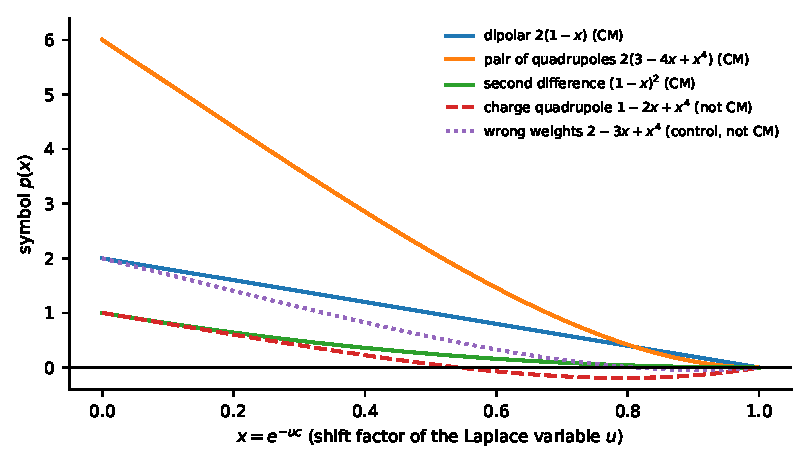
\includegraphics[width=0.62\linewidth]{fig_symbols.pdf}
\caption{Tier X illustration (CM-X-0004), code-generated; the minima are floating-point grid values. Laplace symbols $p(x)$, $x=e^{-uc}$, of the combinations of
translates. Reading $p\ge0$ on $(0,1]$ as ``CM'' uses the easy direction of Bernstein--Widder (\lean{laplace_measure}) together with the
representation $t^{-1/2}=\int e^{-ut}u^{-1/2}\pi^{-1/2}du$; reading a negative $p$ as ``not CM'' would need the hard direction and uniqueness
of the representing measure, which are \emph{not} proved here. The Lean proofs do not use symbols: positive cases use differences of
translates (Step~3) and \lean{quadrupole_not_cm} is a direct evaluation at $t=3$. The minima on the plotted grid are \PnSymMinCharge{} at $x=\PnSymXCharge$ (charge
quadrupole) and \PnSymMinWrong{} at $x=\PnSymXWrong$ (control with wrong weights $2,-3,1$).}\label{fig:sym}\end{figure}

\paragraph{Triangular optimality, conditional \tier{A, CM-A-0012, CM-A-0018; C, CM-C-0003}.}
\lean{triangular_optimal} restates upstream: for $g\in\CM$ and every locally finite density-one $C$,
\lean{latticeEnergy g <= energy g C}; it is instantiated for the soft-core Yukawa, stretched exponential,
screened dipolar, Yukawa-spectrum and Coulomb quadrupolar potentials. All of these rest on upstream \tier{A, CM-A-0001},
which is AI-generated and not peer reviewed, and on the fidelity of its definitions. We prove no finiteness of the optimal
energy for these potentials, so for slowly decaying tails the statement can read $\top\le\top$. Physical modelling (rigid,
aligned, classical point charges, no screening beyond the Yukawa factor, no quantum effects) is Tier~C and the
statements say nothing about uniqueness.

\paragraph{Negative controls \tier{A, CM-A-0013}.} Listing~\ref{lst:neg} shows that each of the listed hypotheses bites (the integrability and measurability hypotheses of \lean{laplace} and $c\ge0$ in the translation lemma are \emph{not} covered by a control): $\cos$ is not
$\CM$; $\sqrt t$ is Bernstein but not $\CM$ and $e^{-t}$ is $\CM$ but not Bernstein, so the classes differ; $1/t$ is $\CM$
and positive but not Bernstein and $e^{-1/t}$ is not $\CM$, so the inner function must be Bernstein; the hypothesis
$\psi>0$ cannot be dropped; and $e^{-t}-2e^{-2t}$ is not $\CM$, so mixture weights must be nonnegative.
\lstinputlisting[caption={Negative controls (selected statements, verbatim, \lean{NegativeControls.lean}).},label=lst:neg]{gen/negctl.lst}

\section{Numerics and tooling (Tier X)}\label{sec:num}
Everything here is \tier{X}: it illustrates, screens or measures, and supports no claim.

\paragraph{A 60-digit screen with controls \tier{X, CM-X-0001}.} For \PnScreenN{} potentials the script
\texttt{cm\_numeric\_check.py} evaluates $(-1)^nF^{(n)}(t)$ for $n=0,\dots,7$ at 15 values of $t$ from $10^{-3}$ to
$10^{4}$ with mpmath (60 digits, numerical differentiation) and reports the minimum signed value. A negative value refutes $\CM$
up to differentiation error; a clean grid never proves it. \emph{Controls.} The two positive controls ($t^{-1/2}$,
$e^{-\sqrt t}/\sqrt t$) show no negative value; the four negative controls ($\cos t$, $t^{-1/2}-2(t+1)^{-1/2}$,
$g_1-2g_2$ and the wrong-weights $2f(t)-3f(t+1)+f(t+4)$) all show one, so the screen can say no, including for a defect
as small as \PnMinWrong. \emph{Results.} Of the \PnScreenCand{} candidates, \PnScreenCandNeg{} shows a negative value: the one-quadrupole
field, with minimum \PnMinCharge{} at $n=0$, $t=3.16$ on this (mpmath) grid; the Lean value at $t=3$ is
$1/\sqrt3-1+1/\sqrt7\approx-0.0447$, and on the finer numpy grid of Figure~\ref{fig:prof} the minimum is \PnChargeVal{} at
$t\approx\PnChargeT$ (a different grid, not a different quantity). The seven other candidates, including the pair
interaction, show none, which is consistent with, and never a proof of, their $\CM$ status (the proofs are the Lean theorems).
\begin{table}[!htbp]\centering\scriptsize
\caption{The screen. The minimum signed value of $(-1)^nF^{(n)}(t)$ over $n\le7$ and the 15 grid values of $t$; for clean
rows it is just the smallest positive value (at the grid end), so only the last column is informative.}\label{tab:screen}
\begin{tabular}{@{}llrrrl@{}}\toprule
$F$ & role & min signed & $n$ & $t$ & negative? \\\midrule
\tabinput{gen/table_screen.tex}
\bottomrule\end{tabular}\end{table}

\begin{figure}[!htbp]\centering
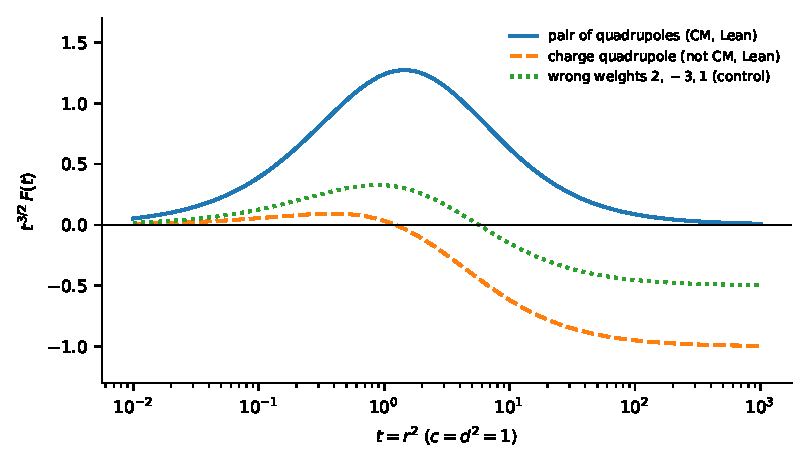
\includegraphics[width=0.62\linewidth]{fig_profiles.pdf}
\caption{Tier X, code-generated (numpy, 600 log-spaced $t$). $t^{3/2}F(t)$ for the interaction of two quadrupoles (Lean: $\CM$),
the field of one quadrupole (Lean: not $\CM$) and the wrong-weights control. At $t=10^3$ the values are \PnFarPair{}
(pair), \PnFarCharge{} (one quadrupole; the far-field limit is $-1$, from $t^{-1/2}-2(t+1)^{-1/2}+(t+4)^{-1/2}\approx2f'(t)=-t^{-3/2}$) and
about $-0.5$ (control); these are values at the grid end, not limits.}\label{fig:prof}\end{figure}

\paragraph{Proof-length measurement and its reading \tier{X, CM-X-0002}.} Method: Lean computes, from the kernel terms, the transitive
closure of declarations in \lean{Programmes.*} and \lean{Autoresearch.*} used by each root theorem. Mathlib, upstream \lean{OAI.*} and the
repository's \lean{Triangular.*} modules are excluded, on both sides. The
script \texttt{proof\_length.py} counts non-blank, non-comment source lines in each declaration's range; overlapping
structure and field ranges are counted twice, on both sides. Neither choice changes the direction of the comparison. The reading of the
counts given below (why the closure grows) is an explanation of a measurement, so it is filed with the measurement as Tier~X and is not a Tier~C claim. Headline
proof (lines, original $\to$ library): H2 \PnHYukawaHeadO$\to$\PnHYukawaHeadL, H1 for $d>0$ \PnHdipolardHeadO$\to$\PnHdipolardHeadL{} (the 23-line proof
was the first version), H1 for every $d$ \PnHdipolaralldHeadO$\to$\PnHdipolaralldHeadL, H3 \PnHKeldyshHeadO$\to$\PnHKeldyshHeadL{}. End to end, however, the closures
grow (Figure~\ref{fig:len}): H2 \PnHYukawaClosO{} (\PnHYukawaDeclO{} declarations) $\to$ \PnHYukawaClosL{} (\PnHYukawaDeclL), H1 \PnHdipolaralldClosO{} (\PnHdipolaralldDeclO)
$\to$ \PnHdipolaralldClosL{} (\PnHdipolaralldDeclL), H3 \PnHKeldyshClosO{} (\PnHKeldyshDeclO) $\to$ \PnHKeldyshClosL{} (\PnHKeldyshDeclL); the union of the three goes from \PnLenOrigUnion{}
lines in \PnLenOrigUnionDecl{} declarations to \PnLenLibUnion{} in \PnLenLibUnionDecl, and with the screened-dipolar and Yukawa-spectrum results
to \PnLenLibNewA{} (\PnLenLibNewADecl) and with the two quadrupolar interactions to \PnLenLibNewB{} (\PnLenLibNewBDecl). The cause is that
\lean{Basic.exp_neg_mul} routes through the earlier Laplace core, which then enters the closure of every exponential-based
result; the Mathlib-only core would avoid it but was not used. The library pays off at the margin: the two new groups
of results add 22 and 21 lines. \textbf{We therefore do not claim shorter proofs overall.}
\begin{figure}[!htbp]\centering
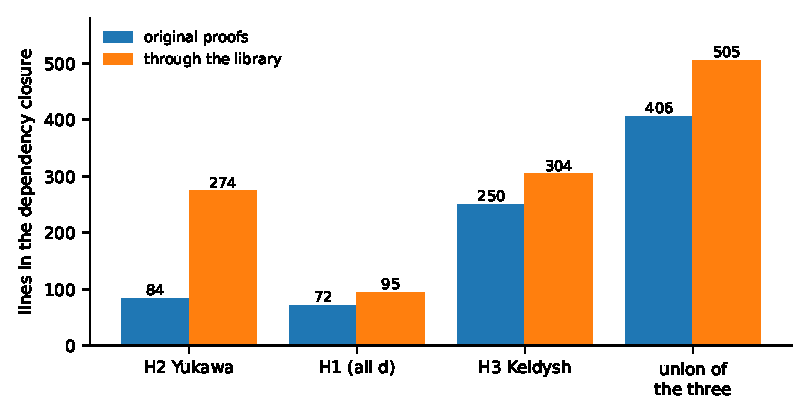
\includegraphics[width=0.55\linewidth]{fig_prooflen.pdf}
\caption{Tier X, code-generated from \texttt{proof\_length.json}: lines in the dependency closure, original proofs versus through the
library.}\label{fig:len}\end{figure}

\paragraph{rusty-SUNDIALS and LeanFlow: no change in this lane.} P3 is a Lean infrastructure lane. Complete monotonicity is a
symbolic property, so a CVODE integration would test nothing here, and the only numerics are the screen above, written
directly in mpmath. No branch of rusty-SUNDIALS exists for P3, no change to LeanFlow was made, and there are therefore no
commit SHAs to report; the AutoevolveAI files are uncommitted on base commit \texttt{\PnBaseShort} of this
worktree (the sha256 values of the Lean sources are in Section~\ref{sec:repro}). Improving rusty-SUNDIALS or LeanFlow
\emph{via} this library (for example an interval-arithmetic CM check) is future work, not a result.

\section{Claim ledger}\label{sec:ledger}
Every claim above is filed in \texttt{ledger/ledger.json} (35 claims: 20 Tier~A, 5 L, 6 C, 4 X) with a content-addressed
evidence blob (verbatim axiom lines and source hashes for A; verbatim excerpts for L; the argument for C; result files with
\texttt{claim\_licence=false} for X). The Elenchus gate \texttt{tools/ledger.py} was run with \texttt{--evidence-dir}
(\texttt{ledger/gate\_output.txt}): \textbf{\PnGateBlock{} blocking findings and \PnGateFlags{} flags, exit code \PnGateExit}; the non-zero exit
code is due to the flags \texttt{LEDGER\_UNAUDITED\_TIER\_A} alone, one for each Tier~A row whose statement adequacy no person has
audited. A first run found one blocking tier inversion: a Tier~C row (the reading of the proof-length counts) depended on a Tier~X measurement. The first repair deleted the dependency edge, which only hid the inversion; the audit restored the edge and the gate then blocked again. The reading is now merged into the Tier~X row CM-X-0002, so no Tier~C row depends on a Tier~X row. The gate checks bookkeeping and cannot say that a claim is true. Of the five Tier~L rows, only the Salazar Theorem~2.3 excerpt is a theorem statement; \texttt{citation\_check.py} accepted it and refused a tampered control. CM-L-0001, 0002, 0003 and 0005 are definitions, prose or policy text, are Tier~L by convention, and were not run through \texttt{citation\_check.py}. \texttt{elenchus\_check.py} could not run on the Lean files (default toolchain, no project search path: COMPILE\_ERROR) and skipped the \texttt{.py} files (no \texttt{CONTROL\_INPUTS}); it gave no verdict, which is not a pass. Of the claims, the
upstream theorem (CM-A-0001) and every optimality statement (CM-A-0012, CM-A-0018) are conditional on AI-generated, unreviewed
work.

\section{Limitations}\label{sec:lim}
\begin{itemize}\itemsep0pt
\item \textbf{No human audit.} The proofs and statements were produced by one AI pipeline and then rebuilt and axiom-checked by an independent AI audit (all 11 files, 167 constants, 0 off the allowlist, planted controls caught; see the disclosure). That audit did not rebuild the upstream openai/math or Mathlib oleans. No person has audited statement adequacy: the 20 Tier~A rows keep their \texttt{LEDGER\_UNAUDITED\_TIER\_A} flags.
\item \textbf{Conditionality.} All optimality corollaries depend on upstream openai/math (AI-generated, not peer reviewed); Keldysh-type tails make them read $\top\le\top$.
\item \textbf{Preregistration versus outcome} (P3, committed before the attempt): core closure (prior 0.8) done; composition with Bernstein functions (prior 0.5) done; Fourier criterion (prior 0.3) not attempted; Stieltjes mixtures not done; the ``Mathlib-PR-ready branch'' goal was not met; the kill rule ``two budgets per lemma'' is not reported on (no lemma is recorded as having been abandoned).
\item \textbf{Scope of the library.} Domain $(0,\infty)$ only; $C^\infty$, not analytic; no hard Bernstein--Widder, no pointwise limits, no arbitrary CM mixtures, no Stieltjes mixtures, no Fourier criterion (preregistered, prior 0.3, not attempted).
\item \textbf{Not a Mathlib contribution.} A different formalisation (\lean{AbsolutelyMonotoneOn}) already exists; the main library imports repository and upstream modules; the Mathlib-only core duplicates code and covers only part; linters were not run; names were checked only against the pinned Mathlib.
\item \textbf{No shorter proofs end to end} (Section~\ref{sec:num}); the weakened Laplace hypothesis is not exercised by H3.
\item \textbf{No novelty claim.} Closure properties are elementary; no literature search for novelty was made; subordination is attributed, not located in the monograph~\cite{ssv}.
\item \textbf{Physics} (quadrupoles, screened excitons) is rigid, aligned, classical and unscreened apart from the Yukawa factor; the pair counting is Tier~C.
\item \textbf{Tier X} evidence is a screen with 60-digit numerical differentiation on a coarse grid; it never proves $\CM$.
\item \textbf{No rusty-SUNDIALS or LeanFlow improvement} was made in this lane.
\item \textbf{Infrastructure.} An anecdotal first cold compile of \lean{Basic} took 872.6 s (disk contention; the figure comes from the lane's \texttt{LIBRARY.md} only, its log was overwritten, and it supports no claim); the Lean files are uncommitted in the repository.
\end{itemize}

\section{Reproducibility}\label{sec:repro}
Toolchain: Lean 4.34.1, Mathlib \texttt{\PnMathlibSha}, openai/math \texttt{fd4aeeb2ee4fc729c18d98444fed42fd0529eeeb} (pinned copy).
AutoevolveAI base commit \texttt{9d245742c1655852103abb28f585e21af54851e6}; the files below are uncommitted at the time of writing.
\begin{itemize}\itemsep0pt\footnotesize
\item \texttt{Basic.lean}: \texttt{eaebc8f68fcab5cc53719f8e7c90ef9e2e4ffe0ce2235a792808c2c85ee10c52}
\item \texttt{Bernstein.lean}: \texttt{9e192c438a949b6d76403135b295a82f93d9918ed00121c630487e9dd909f39d}
\item \texttt{Laplace.lean}: \texttt{fc721ec52eb51e97523e6c07b4d1b3624f608254c28b0a9477f09809c0aa952c}
\item \texttt{Limits.lean}: \texttt{04819006b336f37ca54f6e8459d29c7d9461e17462985ea2f257110282ba78fc}
\item \texttt{Examples.lean}: \texttt{27994bc788426556f45c62674412e36242e108d0e7ea6302506dbc8f8a6a9d39}
\item \texttt{Corollaries.lean}: \texttt{45e2ff5f4e8562f71ad4d36d1c85e384fe3c23060ef01b63e876b93972ed319f}
\item \texttt{NegativeControls.lean}: \texttt{83f5de212ee3f6ad2f2cfb169238c0e1b80a0d3c79af91f69187a47a1661772e}
\item \texttt{MathlibOnly.lean}: \texttt{d0da3c865357431db3817ae7f800c89e9f1289103cdbb7f08fb2184e4b32685d}
\item \texttt{MathlibOnlyBridge.lean}: \texttt{40c0d8be82caacc70e83ba25bfce46fb25e2bc0a31e3f26c27cbdf172cc6e7e0}
\item \texttt{Applications.lean}: \texttt{a6a0d17048eb3e2dd56ee0837e5f688f027b7beecb6cd275e5b5ceb45dceb83f}
\item \texttt{Controls.lean}: \texttt{1469ffd336424ef3dc784a5d65281e4c3e1d943563083cb622c083690c435fce}

\end{itemize}
\begin{lstlisting}[basicstyle=\ttfamily\tiny]
taskset -c 4-7 python3 scripts/certified_numerics/lean_pinned.py compile formal_cert/Programmes/CompletelyMonotone/<M>.lean \
  --olean Programmes.CompletelyMonotone.<M> --json-out results/programmes/2026-10-25/P3/compile_logs/<M>.json
  (order: Basic; Bernstein, Laplace, Limits; Examples, Corollaries; NegativeControls, MathlibOnly; MathlibOnlyBridge; Applications;
   Controls without --olean)
python -I results/programmes/2026-10-25/P3/gate.py
python -I results/programmes/2026-10-25/P3/applications/cm_numeric_check.py out.json     # Tier X screen
python -I papers/prog_cm_bernstein_library/gen_inputs.py                                  # numbers, listings, figures
python -I papers/prog_cm_bernstein_library/ledger/build_ledger.py ; python -I papers/prog_cm_bernstein_library/ledger/run_gate.py
pdflatex main.tex (twice)
\end{lstlisting}
Paper-stage recompile logs are in \texttt{ledger/recompile/}. All code, data and logs are in this directory and in
\texttt{results/programmes/2026-10-25/P3/}.

\begin{thebibliography}{99}\footnotesize
\bibitem{oai} OpenAI, \emph{Universal optimality of the triangular lattice}, OpenAI Math release, github.com/openai/math,
commit \texttt{fd4aeeb2ee4fc729c18d98444fed42fd0529eeeb} (2026). AI-generated; not peer reviewed.
\bibitem{ps} M.~Petrache, S.~Serfaty, \emph{Crystallization for Coulomb and Riesz interactions as a consequence of the
Cohn--Kumar conjecture}, arXiv:1908.09714v3 (2019).
\bibitem{ck} H.~Cohn, A.~Kumar, \emph{Universally optimal distribution of points on spheres}, J. Amer. Math. Soc. \textbf{20}
(2007), 99--148, arXiv:math/0607446.
\bibitem{sal} D.~S.~P. Salazar, \emph{Bernstein functions at work: coalescents, copulas, and subordination}, arXiv:2607.04467v1 (2026);
used only for the definitions (Def.~2.1, p.~4), for the statement of the Bernstein--Widder theorem (Thm~2.3, p.~5) and for the name ``Bochner subordination'' (p.~2).
\bibitem{ssv} R.~L. Schilling, R.~Song, Z.~Vondra\v{c}ek, \emph{Bernstein Functions: Theory and Applications}, 2nd ed., de Gruyter, 2012.
Existence of the monograph was confirmed through its publisher record and through~\cite{sal}; its theorem on composition was
\emph{not} consulted or located.
\bibitem{widder} D.~V. Widder, \emph{The Laplace Transform}, Princeton University Press, 1941 (as cited in the Mathlib
bibliography and in~\cite{ck} p.~101); not consulted.
\bibitem{mlam} Mathlib, \texttt{Mathlib/Analysis/Calculus/AbsolutelyMonotone.lean} (M.~R. Douglas, 2025), at the pinned commit
\texttt{d13f23b723b8a846827a245b89c10fc7d3f11612}.
\bibitem{mlpolicy} Lean community, \emph{How to contribute}, section ``Use of AI'', leanprover-community.github.io/contribute/index.html,
read 2026-10-25.
\bibitem{d2} X.~Callens, \emph{Riesz-energy, finiteness and every-density corollaries of the openai/math planar
universal-optimality theorem, kernel-checked in Lean 4}, doi:10.5281/zenodo.23285631 (2026).
\bibitem{uot} X.~Callens, \emph{Planar universal optimality, tiered}, preprint v2, doi:10.5281/zenodo.23293429 (2026).
\bibitem{txt} X.~Callens, \emph{The Triangular Lattice and Universal Optimality} (textbook), doi:10.5281/zenodo.23295142 (2026).
\bibitem{dip} X.~Callens, \emph{The bilayer dipolar-exciton interaction is completely monotone in $r^2$: kernel-checked
triangular-lattice corollaries at every density and an exact-Ewald CVODE consistency study}, doi:10.5281/zenodo.23646103 (2026).
\bibitem{yuk} X.~Callens, \emph{The triangular lattice minimises the planar Yukawa energy at every density and for every finite
mixture of screening lengths}, doi:10.5281/zenodo.23646105 (2026).
\bibitem{kel} X.~Callens, \emph{The Rytova--Keldysh interaction is a positive Gaussian mixture: kernel-checked admissibility
for planar universal optimality and Keldysh-jellium Madelung energies of TMD Wigner lattices}, doi:10.5281/zenodo.23646107 (2026).
\bibitem{sig} X.~Callens, \emph{A cutoff-independent enstrophy bound for the $\sigma=3$ dispersive dyadic shell model},
doi:10.5281/zenodo.23646111 (2026); sibling preprint of the same programme, not used mathematically here.
\bibitem{bog} X.~Callens, \emph{The Bogoliubov structure factor under the dual-scale envelope $\sqrt{k/2k_s}$},
doi:10.5281/zenodo.23646117 (2026); sibling preprint, not used mathematically here.
\end{thebibliography}
\end{document}
